\documentclass{bioinfo} 
\copyrightyear{2016} \pubyear{2016}
\access{Advance Access Publication Date: Day Month Year}
\appnotes{Original Paper} 
\usepackage{amsmath, amssymb}
    \allowdisplaybreaks 
\usepackage{graphicx}
\newtheorem{thrm}{Theorem} 
\usepackage[
    colorlinks, linkcolor={blue}, citecolor={blue},
    urlcolor={blue}]{hyperref} 
%% Option 1 URW Garamond (free any latex distribution): 
%% =-=-=-=-=-=-=-=-=-=-=-=-=-=-=-=-=-=-=-=-=-=-=-=-=-=-
%    \usepackage[urw-garamond]{mathdesign} 
%    \usepackage[T1]{fontenc} 
%% Option 2: Classic Garamond (requires .pfb sources)
%% =-=-=-=-=-=-=-=-=-=-=-=-=-=-=-=-=-=-=-=-=-=-=-=-=-=-
%    \usepackage[T1]{fontenc} 
%    \usepackage{sabon}
%    \usepackage[italic,defaultmathsizes]{mathastext}
%%    % mdugm.sty magic bellow --- !!!
%    \SetSymbolFont{letters}{normal}{OML}{mdugm}{m}{it} 
%% Option 3 (Times via MathTimes Pro)
%% =-=-=-=-=-=-=-=-=-=-=-=-=-=-=-=-=-=-=-=-=-=-=-=-=-=-
%   \usepackage[subscriptcorrection]{mtpro} 
%       \DeclareMathSizes{8}{7.15}{5.2}{4.2}
%    \usepackage[mtpcal]{mtpb}
\DeclareMathAlphabet{\txcal}{U}{tx-cal}{m}{n}
\usepackage[scaled=1.1]{rsfso}
\renewcommand*\ttdefault{txtt}
\usepackage{url}
    \def\UrlFont{\tt}
%
\usepackage{algorithm}
\usepackage[noend]{algpseudocode}
\makeatletter
  \def\BState{\State\hskip-\ALG@thistlm}
\makeatother
\renewcommand*\copyright{\textcopyright}
\newcommand{\CC}{C\nolinebreak\hspace{-.05em}\raisebox{.4ex}{\tiny
    +}\nolinebreak\hspace{-.15em}\raisebox{.4ex}{\tiny +}}
\newcommand{\Mord}{\mathcal{M}_N}
%=-=-=-=-=-=-=-=-=-=-=-=-=-=-=-=-=-=-=-=-=-=-=-=-=-=-=-=-=-=-=-=-=-=-
\begin{document}
\firstpage{1}
%\subtitle{}
\title[empirical Bayesian NMF]{signeR: An empirical Bayesian approach
  to mutational signature discovery}
\author[Rosales, R. A. and Drummond, R. D.~\textit{et~al}.]{
    Rafael A. Rosales\,$^{\text{\sfb 1,}\dagger}$, 
    Rodrigo D. Drummond\,$^{\text{\sfb 2,}\dagger}$, 
    Renan Valieris\,$^{\text{\sfb 2}}$,
    Emmanuel Dias-Neto\,$^{\text{\sfb 3,4}}$, 
    Israel T. da Silva\,$^{\text{\sfb 2,5}*}$}
\address{% 
   $^{\text{\sf 1}}$Departamento de Computa\c{c}\~ao e
   Matem\'atica, Universidade de S\~ao Paulo, SP 14040-901, Brazil, 
   $^{\text{\sf 2}}$Laboratory of Bioinformatics and Computational 
   Biology, A. C. Camargo Cancer Center, SP  01509-010, 
   Brazil, $^{\text{\sf 3}}$Laboratory of Medical Genomics,
   A. C. Camargo Cancer Center, SP 01509-010, Brazil, $^{\text{\sf  4}}$Laboratory of Neurosciences (LIM27),
   Department and Institute of Psychiatry, Faculty of Medicine, University of S\~ao Paulo, SP 05403-903, Brazil,
   $^{\text{\sf 5}}$Laboratory of Molecular Immunology, The
   Rockefeller University, NY 10065, USA\\[1em]
   {\normalsize $^{\dagger}$The authors wish it to be known
   that, in their opinion, the first two authors should be regarded
   as joint First Authors} 
}
\corresp{$^\ast$To whom correspondence should be addressed.} 
\history{Received on XXXXX; revised on XXXXX; accepted on XXXXX} 
\editor{Associate Editor: XXXXXXX} 
\abstract{%
\textbf{Motivation:} Neoplastic alterations found in
eukaryotic cells may result from mutagenic agents that produce
particular mutation signatures.  These signatures can be used to
understand cancer origins and provide a unique opportunity to group
tumor types that share the same origins and result from similar
processes. Mutational signatures have been identified from high
throughput sequencing data generated from cancer genomes by using
non-negative factorisation (NMF) techniques.  Current methods are
based on optimisation techniques and are strongly sensitive to initial
conditions due to high dimensionality and non-convexity of the NMF
paradigm. An important question in this context consists in the
determination of the actual number of signatures that best represent
the data. The extraction of mutational signatures from high-throughput
data still remains a daunting task.
\\
\textbf{Results:} Here we present a new method for the statistical
estimation of mutational signatures based on an empirical Bayesian
treatment of the NMF model. While requiring minimal intervention from
the user, our method addresses the determination of the number of
signatures directly as a model selection problem. In addition, we
introduce two new concepts, of significant clinical relevance for
evaluating the mutational profile: the differential exposure score and
the posterior classification. The advantages brought by our approach
are shown by the analysis of real and synthetic data sets. The later
are used to compare our approach against two alternative methods
mostly used in the literature and with the same NMF parametrisation as
the one considered here. Our approach is robust to initial conditions
and more accurate than competing alternatives. It also estimates the
correct number of signatures even when other methods fail. Results
obtained in the analysis of a publicly available data set formed by
somatic mutations from 21 breast cancers are consistent with current
knowledge.
\\
\textbf{Availability and implementation:} \texttt{singeR} is
implemented in R and C++, and is available as a R package at 
\url{https://github.com/rvalieris/signeR}\\
 \textbf{Contact:} itojal@cipe.accamargo.org.br\\
\textbf{Supplementary information:} Supplementary data are available
at \textit{Bioinformatics} online.
}
\maketitle
\section{Introduction}
Cancer is a collection of diverse pathological entities that harbour
and probably derive from a complex collection of genomic
alterations. Today, it is widely accepted that the accumulation of
these alterations, including somatic mutations, is one of the major
causes of the malignant transformation, triggering the expansion of
tumour cell clones. As tumors evolve, these mutations are found across
many genomic loci, but also tend to preferentially affect certain
pathways (\citealp{CCSS}). The diversity and complexity of somatic
mutational processes in these clones is a conspicuous feature
orchestrated by DNA damaging agents and repair processes, including
the exposure to exogenous or endogenous carcinogenic/mutagenic agents,
retro-insertion of endogenous retroviruses, defects in DNA mismatch
repair enzymes and enzymatic modifications of the DNA among others
(\citealp{RG}). The actual identification of the underlying mutational
processes is central to an understanding of cancer origin and
evolution (\citealp{ANat, AS, HEN, RG}).


Most somatic mutations include single base substitutions,
insertions and deletions, rearrangements and copy number variations
(CNV). Single base substitutions fall into one of six possible base
changes, namely \texttt{C:G}$>$\texttt{A:T},
\texttt{C:G}$>$\texttt{G:C}, \texttt{C:G}$>$\texttt{T:A},
\texttt{T:A}$>$\texttt{A:T}, \texttt{T:A}$>$\texttt{C:G} and
\texttt{T:A}$>$\texttt{G:C}. According to \cite{A}, this set may be
further enlarged by including the $5'$ and $3'$ neighbouring bases of
each substitution site, leading to an alphabet $\txcal A$ with 96
trinucleotide mutation types. More generally, the definition of
$\txcal A$ could in principle accommodate mutations of various other
kinds
%such as indels, rearrangements, copy number changes 
and even wider neighbouring contexts. Once $\txcal A$ is properly
defined, the counts for the mutations found in $G$ different genomes
are assembled into a $K\times G$ matrix $M$ with $K = |\txcal A|$. An
crucial assumption consists in viewing the counts in $M$ as the
additive effect of $N$ mutational processes, each defined as a
$K\times 1$ vector of mutational rates. The later defines what is
known as a mutational signature. More precisely, the mutations across
all genomes result as the linear combination of $N$ basis vectors of
dimension $K\times 1$, with mixture coefficients defined by $N$
exposure vectors of dimension $1 \times G$. If the basis vectors are
merged into a $K\times N$ matrix of signatures $P$, and the
coefficient vectors into a $N\times G$ matrix of exposures $E$, then
the data can be simply factored as $M=PE$. An example of this is shown
in Figure~\ref{fig:toyNMF}.

\begin{figure*}
  \centering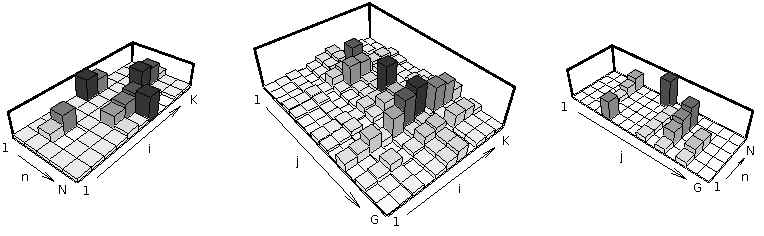
\includegraphics[width = 13.5cm]{figs/f_bw_t}
  \caption{\textrm{%
   A factorisation for a mutation counts matrix $M$. The
   mutation matrix shown at the centre is defined over an alphabet
   with $K = 11$ symbols, $1 \leq i \leq 11$, and $G = 15$ genomes,
   $1\leq j\leq 15$. The matrices at the left and the right
   represent respectively a signature and an exposure matrix $P$ and
   $E$, obtained for a factorisation with rank $N = 5$.
  }
 }
 \label{fig:toyNMF}
\end{figure*}

For any given mutation-count matrix there are essentially two
interrelated questions that should be addressed: 1. the determination
of the underlying signatures and exposures to best account for the
observations, and 2. the determination of the actual number of
signatures $N$. \cite{NCell} and \cite{A} addressed the first issue by
using nonnegative matrix factorisation (NMF) techniques. NMF as
conceived by \cite{LS} finds the factors $P$, $E$ that approximately
solve the following non-convex optimisation problem
\begin{equation}
  \label{eqn:NMF}
    \min_{P\geq 0,\ E\geq 0}\|M - PE\|,
\end{equation}
for a given fixed rank $N$ and an appropriately chosen norm.
To deal with the second question, \cite{NCell} and \cite{A}
perform the factorisation of the same data for various ranks, namely
for $1 \leq N \leq \min\{K, G\}-1$. The rank is then determined rather
indirectly by studying the clustering properties of the obtained
factors via a criterion developed by \cite{BTGM} or by using the 
residual sum of squares, \cite{HMSG}.

An alternative approach to mutational signature discovery, and to NMF
in general, follows from a statistical interpretation of the problem
posed by (\ref{eqn:NMF}) in which $M$ is assumed to be a random matrix
distributed according to a member of the exponential family
parameterised by $P$ and $E$. The optimisation problem posed by
(\ref{eqn:NMF}), under the norm induced by a specific Bregman
divergence (see \citealp{BMD}), turns to be equivalent to the maximum
likelihood estimation of $P$ and $E$.  For instance, if $M$ is Poisson
distributed with rate $PE$, then the likelihood maximisation with
respect to $P$ and $E$ is equivalent to the minimisation of
(\ref{eqn:NMF}) under the norm defined by the Kullback-Leibler
divergence. The maximisation of a Gaussian likelihood is equivalent to
the minimisation under the Frobenius norm. A key aspect of this
perspective is that it allows to treat the determination of the
factorisation rank $N$ as a model selection problem. The statistical
interpretation was developed by \cite{C}, \cite{FC} and \cite{SWK} in
the general NMF context and then considered by \cite{FICMV} for the
mutational signature application. \cite{FICMV} modelled $M$ as Poisson
distributed and then considered the estimation of $P$ and $E$ by using
an expectation maximisation (EM) algorithm. The number of mutational
signatures where estimated by considering an (unnecessary) saddlepoint
approximation to the Bayesian information criterion (BIC). Recently,
\cite{STMS} and \cite{RMHTS} also considered a statistical approach to
the determination of mutational signatures. The former, however,
considers a different NMF parametrisation in which the features
composing each mutation type in $\txcal A$ are assumed
independent. The latter considers the simpler problem of the
estimation of $E$ for given $M$, $P$ and $N$.

In this article we consider an empirical Bayesian treatment to the NMF
model as initially described by \cite{A} for the estimation of
mutational signatures. Following \cite{FICMV}, our model also
incorporates the genome frequencies of the triplets where each
mutation type in $\txcal A$ can occur, which are known as
opportunities. These enter the model as a matrix of weights $W$,
leading to observations generated at rate $PE\circ W$ with $\circ$ as
Hadamard's element wise matrix product. Both, the effectiveness and
the advantages of our method are shown by using real and synthetic
data sets.

\section{Approach}
\subsection{Hierarchical model}
\subsubsection{Likelihood and latent variables}
Let $p_{in} = (P)_{in}$ be the $i,n$-entry of $P$ and likewise let
$e_{nj} = (E)_{nj}$ and $w_{ij} = (W)_{ij}$.  The random variables
$M_{ij}$ are assumed to be independent and Poisson distributed with
rates 
$
  (PE\circ W)_{ij} = w_{ij}\sum_{n=1}^N p_{in}e_{nj}.
$
For a given sample of $M$, say $m$, this formulation is sufficient to
define the likelihood function $\mathcal L(\theta, W; m)$ if one
identifies the matrices $P, E$ as model parameters $\theta$, for
$\theta \in \Theta = \mathbb R_+^{K\times N}\times \mathbb
R_+^{N\times G}$. The opportunities are either known or set to $W =
\mathbf{1}$, and hence regarded as fixed parameters. To simplify
notation we omit any further reference to $W$. An expression for
$\mathcal L(\theta; m)$ is presented as supplementary material by the
equation ($s_1$).

This relatively simple model allows for a latent variable
representation in which the observed counts are expressed as the sum
of $N\geq 1$ independent Poisson variables
\begin{equation}
  \label{eqn:latent_representation}
   M_{ij} = Z_{i1j} + Z_{i2j} + \ldots + Z_{iNj},
\end{equation} 
each with rate respectively equal to $p_{in}e_{nj}w_{ij}$. This
description is an immediate consequence of the properties of sums of
independent Poisson random variables. Biologically, this accounts for
the observation that the total number of mutations of a specific type,
say $(i,j)$, arise as the linear combination of $N$ mutational
processes $Z_{inj}$, $n = 1, \ldots, N$. From a statistical
perspective, (\ref{eqn:latent_representation}) enables a data
augmentation scheme that becomes instrumental for a Bayesian treatment
to NMF. As observed by \cite{C}, this allows the implementation of
several powerful techniques such as the Expectation Maximisation (EM)
algorithm, Markov chain Monte Carlo (MCMC) and variational Bayesian
approximations.  Our approach to NMF fully exploits the data
augmentation scheme defined by~(\ref{eqn:latent_representation}).
Hereafter we denote by $Z$ the random tensor $\{Z_{inj}: 1\leq i\leq
K, 1\leq n \leq N, 1\leq j\leq G\}$ and then let $z$ be a generic
value for $Z$.

\subsubsection{Priors and hyperpriors} 
We consider conjugate priors for the matrices $P$ and $E$ by modelling
each of their entries as being independent Gamma distributed random
variables. Specifically, $p_{in}$ is Gamma distributed with shape
$\alpha_{in}^p + 1$ and rate $\beta_{in}^p \geq 0$ for $\alpha_{in}^p
\geq 0$. Likewise, $e_{nj}$ are Gamma with shape $\alpha_{nj}^e+1$ and
rate $\beta_{nj}^e \geq 0$ for $\alpha_{nj}^e \geq 0$. Shape
parameters are shifted by 1 to ensure bounded values for the Gamma
densities, improving stability of the computational methods described
in subsequent sections. Let $A_p$ and $B_p$ be $K\times N$ matrices
respectively with entries $\alpha_{in}^p$ and $\beta_{in}^p$ and
$A_e$, $B_e$ be $N\times G$ matrices with elements $\alpha_{nj}^e$ and
$\beta_{nj}^e$, and then let $\psi = (A_p, B_p, A_e, B_e)$ denote the
hyperparameters.


A further hierarchy in our model is set by considering the
distributions for the hyperparameters $\psi$. By conjugancy to the
prior, we define the entries of $B_p$ as being independent and
distributed according to a common Gamma distribution with shape and
rate $a_p > 0$, $b_p > 0$. Similarly, the elements of $B_e$ are Gamma
distributed with shape $a_e>0$ and rate $b_e>0$. The situation for the
matrices $A_p$ and $A_e$ is however different. While a Gamma
distribution for the entries of $A_p$ and $A_e$ is conjugate to the
Gamma prior (see \citealp{M}), the resulting full conditional
distribution necessary to draw inferences about $A_p$ and
$A_e$ does not has a standard form.  This fact has long been
recognised in the Poisson hierarchical model (\citealp{GMS93}) and may
be dealt with by choosing any parametric family of distributions with
the appropriate support. Here we take the elements of $A_p$ and
$A_e$ as independent and exponentially distributed with rates
$\lambda_p > 0$ and $\lambda_e > 0$.  Let $\eta$ be the vector of
hyperprior parameters $(a_e$, $b_e$, $a_p$, $b_p$, $\lambda_p$,
$\lambda_e)$ defined on $\Lambda = (0, \infty)^6$.
% $\psi \in \psi = \mathbb R_+^{K\times N}\times \mathbb R_+^{N\times
% G}\times \mathbb R_+^{K\times N}\times\mathbb R_+^{N\times G}$ and 
% $z \in \txcal Z = \mathbb Z_+^{K\times N\times G}$.

\subsection{Bayesian treatment}
We follow an empirical Bayesian approach in which the parameters
$\theta$, the hyperparameters $\psi$ and the hyperprior parameters
$\eta$ are all estimated from the data.  Inferences about the
mutational signatures and their exposures are driven by the posterior
distribution for the NMF model by combining MCMC and EM techniques as
encouraged by \cite{C01}. Specifically, for a given value of $\eta$ we
consider a Metropolized Gibbs sampler targeted towards the conditional
posterior $\pi(\theta|M, \eta)$. This entails the iterative generation
of a sequence of samples $\big(Z^{(r)}, \theta^{(r)},
\psi^{(r)}\big)$, $r \geq 1$, from the set of full conditional
distributions
\begin{gather*}
   Z^{(r+1)} \sim \pi(Z| \theta^{(r)}, \psi^{(r)}, M, \eta), \quad
   \theta^{(r+1)} \sim \pi(\theta| Z^{(r+1)}, \psi^{(r)}, M, \eta), \\
       \text{and}\quad
   \psi^{(r+1)} \sim \pi(\psi| Z^{(r+1)}, \theta^{(r+1)}, M, \eta).
\end{gather*}
These samples are used to update the value of $\eta$ via a stochastic
EM step and the later is then used to draw a subsequent sequence of
samples for $Z$, $\theta$ and $\psi$. The successive iteration of
these steps defines a convergent sequence $\big(\eta^{(u)}\big)$, $u
\geq 1$, allowing the estimate $\hat\eta = \eta^{(U)}$ for
sufficiently large $U$. A final set of MCMC samples for $Z$, $\theta$
and $\psi$ drawn by conditioning on $\hat\eta$ provide the following
estimate
\begin{equation}
 \label{eqn:MCEM_estimate}
   \widehat{\pi}(\theta|M, \hat\eta)
 = 
   \frac{1}{R}\sum_{r=1}^R \pi(\theta|Z^{(r)}, \psi^{(r)}, M,
   \eta^{(U)})
\end{equation}
of the required posterior $\pi(\theta|M, \eta)$.

The MCMC samples are used to compute estimates and all other related
posterior statistics for the signatures and their exposures. The
sampled matrices are first rescaled such that the columns of $P$ sum
to 1 and the product $PE$ is left unaltered. The full set of rescaled 
samples is used to exploit the posterior distribution of those
parameters, allowing to define two novel applications described in
Sections~\ref{sec:DES} and \ref{sec:Class}.  Point
estimates for the signatures and their exposures are considered for
visualisation and comparison purposes. These are computed as the
sample median and denoted hereafter by $\widehat P$ and $\widehat E$
respectively.

Details about the implementation of Gibbs sampler are relatively
standard and are included in Section 2 of the supplementary
material. The following section presents and justifies the MCMC EM  
approach. 

\subsubsection{MCMC EM}\label{sec:MCMCEM}
For a given data sample $m$ and $Z = z$, direct use of Bayes theorem 
allows to  express the marginal likelihood for $\eta$, i.e. the
function $\mathcal L: \Lambda \to \mathbb R$ induced by $\eta 
\mapsto p(M=m|\eta)$, as
\begin{equation}
  \label{eqn:margLik}
  \mathcal L(\eta; m) 
  = \frac{\mathcal L(\eta; m, z, \theta, \psi)}{\pi(z,
      \theta, \psi|m, \eta)}.
\end{equation}
Here $\mathcal L(\eta; m, z, \theta, \psi)$ is 
defined as being equal to  $p(M=m$, $Z=z$, $\theta$,
$\psi|\eta)$ but considered as a function of $\eta$.  This quantity
can be evaluated by observing the conditional decomposition
\[
   \mathcal L(\eta; m, z, \theta, \psi) 
  = 
   p(M=m, Z=z|\theta) p(\theta|\psi)p(\psi|\eta), 
\]
where $p(\theta|\psi)$ and $p(\psi|\eta)$ stand respectively for the
prior and the hyperprior distributions, and $p(M=m, Z=z|\theta)$ is the
complete data likelihood. An expression for the later is included as 
supplementary material by equation ($s_2$). Taking
logarithms and integrating with respect to the posterior distribution
$\pi(Z, \theta, \psi|m, \eta)$ with $\eta = \eta_0$ at both sides of
(\ref{eqn:margLik}) gives 
\begin{align*}
   \mathbb E\big[\ln\mathcal L(\eta; m) \big| \eta_0\big] 
  =\ & 
  \mathbb E\big[\ln\mathcal L(\eta; m, Z, \theta, \psi)
    \big|  \eta_0\big]\\ 
     &-
  \mathbb E\big[\ln \pi(Z, \theta, \psi\,|\,m,\eta)\big| \eta_0\big].
\end{align*}  
This expression is the basic identity on which the EM algorithm is
built and justifies therefore the convergence of the sequence
\begin{equation}
 \label{eqn:EofMCEM}
  \eta^{(u+1)} = \underset{\eta\,\in\, \Lambda}{\text{arg max}}\, 
  \mathbb E\Big[\ln\mathcal L(\eta; m, Z, \theta, \psi)\big|
  \eta^{(u)}\Big], 
  \quad u\geq 0,
\end{equation}
towards the maximum likelihood estimate of $\eta$ for any $\eta^{(0)}
= \eta_0  \in \Lambda$. The integral involved in the above expectation
cannot be computed directly but it may be estimated via Monte Carlo,
leading to the sequence 
\begin{equation}
 \label{eqn:MCEM}
   \hat\eta^{(u+1)}
 = 
    \underset{\hat\eta^{(u)}\,\in\,\Lambda}{\text{arg max}} 
   \bigg\{
    \frac{1}{R}\sum_{r=1}^R 
      \ln\mathcal L\Big(\hat\eta^{(u)}; m, Z^{(r)}, \theta^{(r)},
      \psi^{(r)}\Big)
   \bigg\}.
\end{equation}
The maximisation steps involved in (\ref{eqn:MCEM}) are relatively
simple to implement and further detailed in Section 3.1 of the
supplementary material.


The procedure described is valid because the sampler developed
throughout generates $\big(Z^{(r)}, \theta^{(r)}, \psi^{(r)}\big)$
approximately from the posterior distribution that is actually used to
define the expectation in (\ref{eqn:EofMCEM}), see for instance
\cite{FM}. This rises however the issue as to in what sense
$\widehat\pi(\theta|M, \hat\eta)$ defined by (\ref{eqn:MCEM_estimate})
can be regarded as an estimate for $\pi(\theta|M, \eta)$. The answer
to this is provided by the following result. Let $f(\theta|M, \eta)$
be the density of the posterior distribution $\pi(\theta|M, \eta)$.

\begin{thrm} For any measurable set $B\subseteq \Theta$,
 $\widehat\pi(B|M,\hat\eta)$ converges in total variation
towards $\pi(B|M,\eta)$ as $R, U \to \infty$, that is
\[
   \lim_{U,\ R\to\infty}
   \sup_{B}
    \bigg|
     \int_B
      % \frac{1}{R} \sum_{r=1}^R \pi(\theta|M, \psi^{(r)}, Z^{(r)}, 
      %    \hat\eta^{(U)}) 
     \Big[
       \widehat \pi(\theta|M, \hat\eta) - f(\theta|M,\eta)
     \Big]\, d\theta
    \bigg|
   = 0.
\]
%\[
%    \lim_{R,\ u\to\infty}
%     \big|
%       \widehat\pi(\, B|M, \hat\eta) - \pi(\, B|M,\eta)
%     \big|
%   =
%    0,
%\]
%where converge is with respect to the total variation norm. 
\end{thrm}

The proof to this is included in Section 3.2 of the accompanying 
supplementary material. 

The implementation of the MCMC EM used to estimate $\eta$ and generate
the samples for $(Z, \theta, \psi)$ conditionally on $\eta$ for the
rank $N$ is shown in Algorithm~\ref{alg:mcmcem}. Model parameters
$\theta$ are initialised by sampling from the prior or by considering
the optimisation approach to (\ref{eqn:NMF}), implemented in R via the
NMF package by \cite{GS}. The constants $R_1$, $R_2$ and $U$ are set
to 100, 1000 and 1000, but may also be changed by the user.

\begin{algorithm}
\caption{MCMC EM}\label{alg:mcmcem}
\begin{algorithmic}[1]
%\Procedure{Initialise}{}
\BState $\textbf{Input:}$ $M$, $W$, $N$, \texttt{start}
\BState $\textbf{Initialize}\ \eta, \psi, \theta, Z \textbf{:}$
\State $\textit{u} \gets \text{0}$; $\epsilon \gets 1$
\State $\eta^{(0)} \gets (1, \ldots, 1)$
\State $\psi^{(0)} \gets \psi^{prior} \sim p(\psi | \eta^{(0)})$
%\Comment{hyperprior distribution}
\If {\texttt{start} = ``\texttt{NMF}''} 
\State $\theta^{(0)} \gets \text{NMF}(M/W)$ %\Comment{NMF: \cite{GS}}
\Else
\State $\theta^{(0)} \gets \theta^{prior} \sim p(\theta | \psi^{(0)})$
%\Comment{prior distribution}
\EndIf {$\textbf{end if}$}
\State $Z^{(0)} \gets Z^{conditional} \sim p(Z \mid \theta^{(0)},
\psi^{(0)}, M, \eta^{(0)})$
%\Comment{full conditional}
\State \textbf{Burning phase:} run the Gibbs sampler for $R_2$ 
iterations
\While {$\epsilon > 0.05$ \textbf{and}  $u \leq U$}
\State Iterate the Gibbs sampler to get  $\big(Z^{(r)},
 \theta^{(r)}, \psi^{(r)}\big)$, $1 \leq r \leq R_1$
\State Update $\hat\eta^{(u)}$ according to the MCMC EM 
formula~(\ref{eqn:MCEM})
\State $\epsilon \gets \|\hat\eta^{(u)} -
\hat\eta^{(u-1)}\|_{\infty}$
%\Comment{supremum norm or maximum} 
\State $u \gets  u+1$
\EndWhile {$\textbf{end while}$}
\BState \textbf{Final run:} Set $\hat\eta \gets \hat\eta^{(u)}$ and
iterate the Gibbs sampler to obtain the final sequence of samples
$\big(Z^{(r)}, \theta^{(r)}, \psi^{(r)}\big)$, $1 \leq r \leq R_2$
\end{algorithmic}
\end{algorithm}

\subsection{Model dimension}
The samples for $\theta$ generated by the last iteration of the
MCMC EM analysis are considered for the estimation of the number 
of mutational signatures $N$. To this end let $T = \min\{K, G\} - 1$
and then for each $1 \leq k \leq T$ let
\[
  \text{BIC}_k^{(r)} = 2\ln\mathcal L\big(m;
    \theta^{(r)}_{k}\big) - k(G+K)\ln G, \qquad r =1, \ldots,
    R
\]
with $\theta^{(r)}_k$ as the sequence of sampled signatures and
exposure matrices of rank $k$. It is important to observe that in
contrast to the approach in \cite{FICMV}, the evaluation of the BIC
here does not requires any further approximation because the
likelihood $\mathcal L(\theta^{(r)}_N; m)$ is directly available, see
($s_1$).  Let $\overline{\text{BIC}}_k$ be the median of 
$\{\text{BIC}_k^{(r)}$, $r = 1, \ldots, R\}$. The number of signatures
$N$ is estimated as
\[
   N 
   = 
   \big\{1 \leq k \leq T:  \overline{\text{BIC}}_k \geq
    \overline{\text{BIC}}_q,\ q\neq k \big\}.
\]

The evaluation of the Bayesian information criterion for all
$1\leq k \leq T$ can be expensive for relatively large $T$
because this involves a full MCMC EM analysis at each $k$. The
algorithm~\ref{alg:optN} describes a simple mode finding strategy that 
works for unimodal BIC sequences and reduces the overall computational
cost.  

\begin{algorithm}
\caption{Model Selection}\label{alg:optN}
\begin{algorithmic}[1]
%\Procedure{Initialise}{}
\BState $\delta \gets 2^d$ for $d \in \mathbb{N}$ such that
$\frac{1}{8}T < \delta \leq \frac{1}{4}T$
\State $\mathcal{T} \gets \{1, 1+\delta,1+2\delta, \ldots, T\}$
\State $i \gets 1$
\State $k^* \gets k \gets \mathcal{T}[1]$
\State Compute $\overline{\text{BIC}}_{k^*}$ via Algorithm 1 with $N
\gets k^*$
\While{$k < (k^* + 2\delta)$ \textbf{and}
  $i<length(\mathcal{T})$} \label{coarse_search}
%\Statex \Comment{stop if two consecutively tested ranks show
%$\overline{\text{BIC}}\; \leq \; \overline{\text{BIC}}_{k^*}$}
\State $k \gets \mathcal{T}[i+1]$
\State Compute $\overline{\text{BIC}}_{k}$ via Algorithm 1 with $N
\gets k$
\If{$\overline{\text{BIC}}_k > \overline{\text{BIC}}_{k^*}$} $k^*
\gets k$
\EndIf
\State $i \gets i+1$
\EndWhile {$\textbf{end while}$}
\While {$\delta > 1$} \label{refine_search}
\State $\delta \gets 2^d/2$ 
\State $\mathcal T \gets \{k^*-\delta, k^*,  k^*+\delta\}$
\State $k^* \gets \big\{k \in \mathcal T: \overline{\text{BIC}}_k
\geq \overline{\text{BIC}}_q,\ q \in \mathcal T\big\}$
\EndWhile {$\textbf{end while}$}
\BState \textbf{Final estimate:} $N \gets k^*$
\end{algorithmic}
\end{algorithm}

\subsection{Differential Exposure Score}\label{sec:DES}
The exposure matrices $E^{(r)}$, $1 \leq r \leq R$, keep important
information about the contribution of each signature across the genome
samples. This can be associated with independent knowledge such as
clinical data in order to check how the activity of each mutational
process correlates to the later. In particular, when \emph{a priori}
information motivates the division of samples in two or more
categories, we propose the use of the Kruskal-Wallis test to check
whether exposure values are significantly different among
categories. This test is applied to each sample of the exposure matrix
$E^{(r)}$ generating a set of $p$-values, $p^{(r)}$, $1 \leq r \leq
R$, for each signature. The median of minus the logarithm of these
values defines what we call the \emph{Differential Exposure Score}
(DES). Signatures with a DES above a prescribed level are considered
as differentially active among groups.

\subsection{Genome sample classification}\label{sec:Class} 
The samples $E^{(r)}$, $1\leq r\leq R$, can also be used for the
classification of genomes. The same as in Section~\ref{sec:DES},
assume there exists prior information motivating the
division of samples in two or more categories and suppose there are
genomes for which this information is not available 
(unlabelled samples). Assigning those genomes to one of the categories 
based on their mutational profiles could be of interest, especially
in clinical applications. We propose the use of classification
algorithms, e.g. $k$-Nearest Neighbours to accomplish this task. The
selected algorithm is applied to each sample $E^{(r)}$ in order to
classify the unlabelled genomes according to their exposures to
mutational processes.  This procedure generates a set of possible
classifications for each unlabelled sample, and one can apply a
majority rule to find the final group assignment.  Unlabelled samples
are assigned to a group if there is more than 75\% of agreement among
possible classifications, otherwise they are labeled as
\textit{undefined}. This approach clearly provides a valuable tool
for prognostic.

\section{Methods}
\begin{figure*}[htb!]
 \centering
 \begin{tabular}{c}
  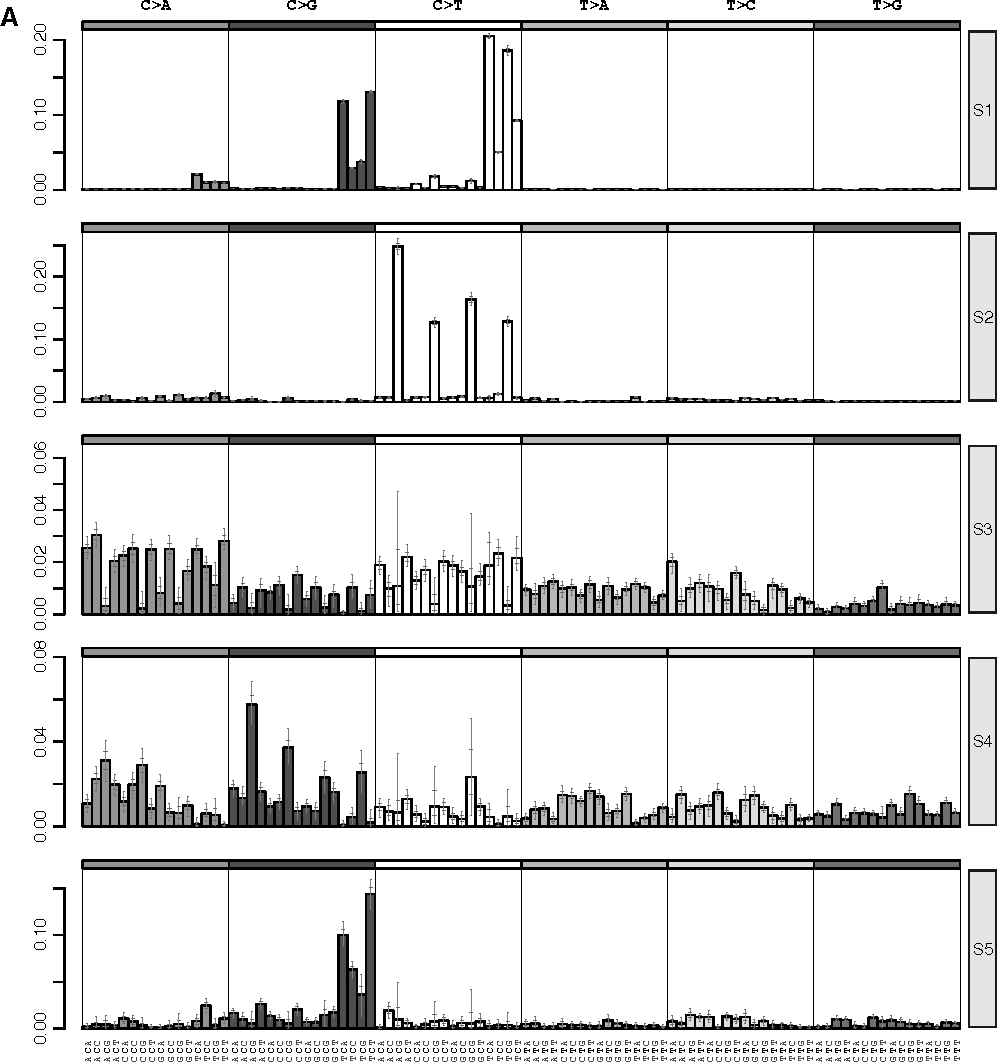
\includegraphics[width=14cm]{figs/Signatures_5_com_Opp_bw} 
  \\
  \begin{tabular}{ccc}
   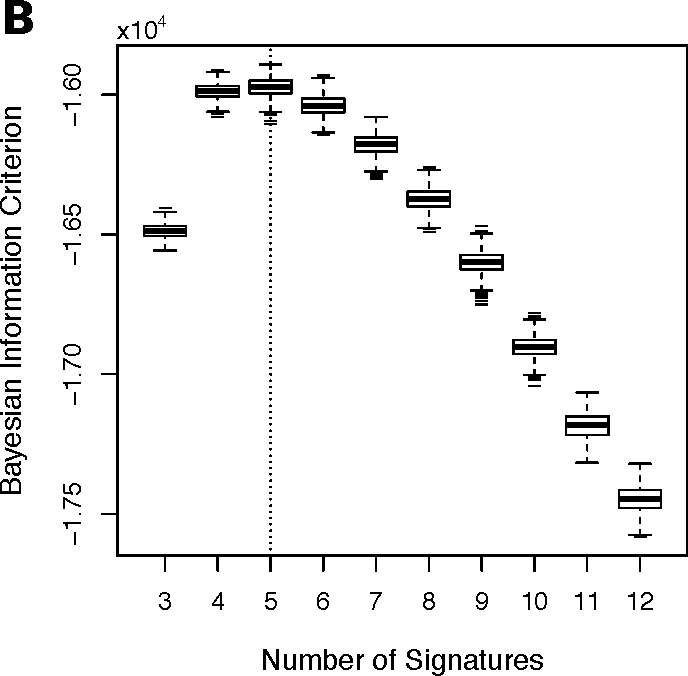
\includegraphics[width=5.5cm]{figs/BICs_21bc_with_Opportunity_5_3to12}
   &
   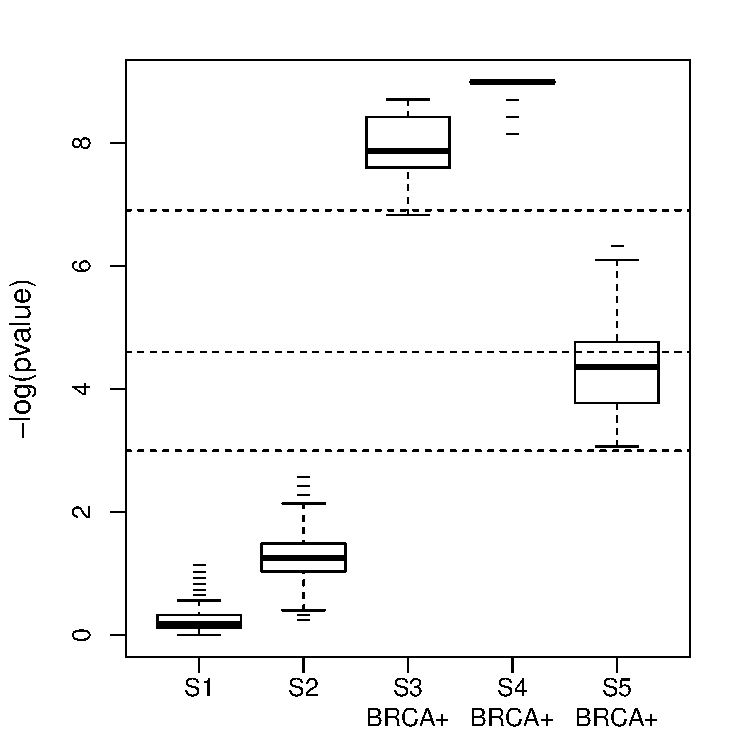
\includegraphics[width=5.5cm]{figs/Diffexp_boxplot_21bc_com_Opp_bw3}
   & 
   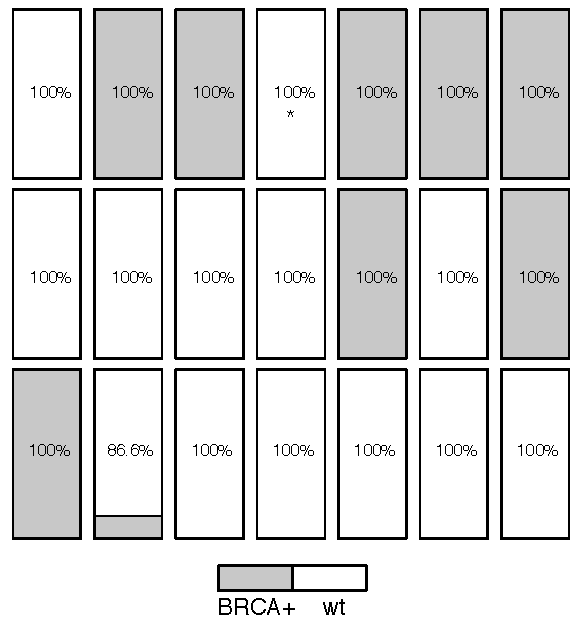
\includegraphics[width=4.5cm]{figs/Classific}
 \end{tabular}
 \end{tabular}
 \caption{\textrm{%
    Results for the 21 breast cancer data. A presents the five
    signatures obtained for the highest NMF model rank according to the
    BIC score presented in B. Signatures are labelled according to the
    order induced by the total signature exposure defined as $\hat e_n =
    \sum_{j} \hat e_{nj}$, with $S_1$ being the most exposed
    signature. Bars are located at the MCMC sample median,
    i.e. $\widehat P$, while other horizontal level marks are located
    at the sample percentiles 0.05, 0.25, 0.75, and 0.95.
    B: Boxplots for the BIC$^{(r)}_k$, $1 \leq r \leq R$, values 
    obtained at various NMF ranks, $N$. C: Differential exposure
    scores - signatures
    showing median of log-$p$-values above thresholds were selected as
    differentially active among groups, and labels show group where they
    were most active.  Dashed horizontal lines are located at 
    the levels 0.05, 0.01 and 0.001. D: Classifications
    obtained for each breast cancer genome based on the remaining 20
    samples. The sample marked as `*' was the only
    misclassification found, `wt' stands for wild type
    \emph{BRCA1}/\emph{BRCA2} condition. Percentages show the
    proportion of agreement among classifications for each genome
    sample.
  }
 }\label{fig:bcancer} 
\end{figure*}
\subsection{Data} The data set containing 183916 somatic point
mutations from 21 breast cancer genomes was obtained from
\url{ftp://ftp.sanger.ac.uk/pub/cancer/Nik-ZainalEtAl}, by following
the instructions in~\cite{NCell}, Table S1. Single base substitutions
where mapped onto trinucleotide sequences by considering the $5'$ and
$3'$ neighboring bases in order to construct a $96\times 21$ matrix of
mutation counts.  The $(i,j)$-th element of the opportunity matrix was
computed as the frequency of the triplets in the $j$-th genome where
the $i$-th mutation can occur. This frequency takes in account the
Copy Number Variations found in the data set by \cite{NCell}. 

\subsection{\texttt{signeR}}
All analyses described here are implemented in the open-source R
language. Low level functions for the generation of random samples
were coded in \CC. The design of our algorithm provides a combination
of speed and low memory overhead enabling the execution on a standard
computer. The stand alone algorithm, \texttt{signeR}, is available at
\url{https://github.com/rvalieris/signeR}. This package allows the 
extraction of the sequence context of somatic variants
necessary to construct the $M$ matrix from VCF files and also
provides a variety of graphics to facilitate the interpretation of
results. Further instructions about how to install and run this
software are included as supplementary material.

\section{Results}
\subsection{The 21 breast cancer data}
The analysis of the 21 breast cancer data made by considering
opportunities revealed 5 distinct signatures
(Figure~\ref{fig:bcancer}.A) that agree well with existing knowledge
as documented in Sanger's catalogue of somatic cancer mutations
(COSMIC, \url{http://cancer.sanger.ac.uk/cosmic/signatures}), and
in \cite{HEN} and \cite{ANat}. The number of signatures necessary to
describe the data was obtained by considering the median BIC value out
of the set of values computed via the MCMC samples. The BIC boxplots
obtained by varying $N$ from 1 to 12 are shown in
Figure~\ref{fig:bcancer}.B. Signatures $S_1$ and $S_5$ (respectively
signature 2 and 13 in COSMIC) are attributed to activity of the APOBEC
family of cytidine deaminases.  Signature $S_2$ (signature 1 in
COSMIC) is associated with a process initiated by the spontaneous
deamination of 5-methylcytosine and correlates with the patient age at 
cancer diagnosis. Signature $S_3$ (signature 3 in COSMIC) is
associated with failure of DNA double-strand break-repair by
homologous recombination, whereas signature $S_4$ has not been
reported previously.

Results for the differential exposure score obtained while grouping
the data into two categories defined by samples with and without
germinative mutations in \emph{BRCA1} and \emph{BRCA2} genes are
presented in Figure~\ref{fig:bcancer}.C. The proteins encoded by the
genes \emph{BRCA1} and \emph{BRCA2} play important roles in
maintaining genomic stability and are involved in a variety of
cellular processes such as damage, signalling and DNA repair
(\citealp{LY}). Disruption of such processes often leads to a rapid
and widespread accumulation of somatic mutations in cancer cells
(\citealp{Ash}). DES highlights three mutational signatures
(Figure~\ref{fig:bcancer}: $S_3$-$S_5$), one is associated with
inactivating mutations in \emph{BRCA1}/\emph{BRCA2} genes ($S_{3}$),
another is implicated with the activity of APOBEC genes ($S_5$). Taken
together, these findings are consistent with existing knowledge and,
at the same time, they reinforce and help demonstrating the failure in
the response to DNA damage by homologous recombination in
BRCA-defective breast cancer. Interestingly, the signature $S_4$ is
preferentially exposed in patients with deletions and mutations in
gene p53 (Tables S.1 and S.2, supplementary material), associated with
more aggressive tumours in triple negative breast cancers
(\citealp{DP}). We observe that the signatures $S_1$ and
$S_2$, which are not differentially exposed, have been reported as
being present in most cancer types by Sanger's catalogue. We conclude
that the DES method is quite effective at revealing genotype-phenotype 
relationships between groups of interest.

A leave-one-out cross-validation strategy was applied to test our
classification approach by examining the same sample categories used
in the DES analysis. This study is motivated by the fact that patients
with mutational profiles similar to those found in genomes with
mutated BRCA genes could respond to treatments targeting defective DNA
double-strand break repair mechanisms (\citealp{Ash}).  Each one of
the 21 genome samples had its label removed and was then subsequently
classified based on the remaining 20 samples.  Results presented in
Figure~\ref{fig:bcancer}.D show that only one sample carrying a
mutation at the \emph{BRCA1} gene was misclassified, thus reinforcing 
the efficacy of our classification approach.

\subsection{Simulation study}
Synthetic data sets mimicking real observations were assembled by
taking a group of four mutational signatures commonly found in breast
cancer genomes. These include the signatures 1, 2, 3 and 13 described
in Sanger's catalogue. Throughout, let $\widetilde P$ denote the
resulting signature matrix.  The exposures are generated by maximising
the likelihood $\mathcal L(\theta; m)$ for a given data sample $m$
with respect to the exposure matrix $E$ by assuming the data as being
generated by $\widetilde P$. The maximisation of the likelihood in
($s_1$) with $P$ fixed at $\widetilde P$ is achieved by using R's 
\texttt{nlopt} package, but it may also be made by using
\cite{LS} multiplicative update algorithm to solve~(\ref{eqn:NMF}). A
matrix of simulated mutation counts $\widetilde m$ is finally
generated by sampling each entry $\widetilde m_{ij}$ from a Poisson
distribution with rate $(\widetilde P\widetilde E\circ W)_{ij}$.

Two synthetic data sets $\widetilde m_1$ and $\widetilde m_2$ were
generated by using the 21 breast cancer data respectively without and
with opportunities, i.e. by setting $W=\mathbf{1}$  or taking $W$
from the real data. The former is used to compare the estimates for 
 $\theta$ produced by
\texttt{signeR} and the method in \cite{A}. The latter was used to
establish a comparison between \texttt{signeR} and the method in
\cite{FICMV}. We refer to these two alternative methods respectively 
as LBA and EMu. The data set $\widetilde m_1$ was analysed 100 times
by both \texttt{signeR} and LBA and $\widetilde m_2$ 500 times by
\texttt{signeR} and EMu. The NMF rank was set to 4 for all analyses
made by LBA. All of the analyses made with \texttt{signeR}
correctly estimated four signatures. Only 51 of the analyses
performed by EMu detected four signatures, the other 449 analyses
estimated three.  The accuracy of each method was compared by the sum
of squared errors between $\widetilde P$ and the estimated signature
matrix $\widehat P$, defined by squaring the Frobenius norm of
$\widehat P - \widetilde P$. This actually led to the consideration of
\[
   \min_k 
   \big\|
       \widetilde P - \widehat P[k]
   \big\|_F^2 
  = 
   \min_k \sum_{in}
     |\widetilde p_{in} - \widehat p_{ik(n)}|^2,
\]
where $\widehat P[k]$ is a permutation of the columns of $\widehat P$
introduced to account for the order in which each method exports the 
signatures. Only those runs where EMu correctly estimated the
dimension of $P$ where included for this analysis. These results are
presented in Figure~\ref{fig:synth_SSE}A., \ref{fig:synth_SSE}.B.
Clearly, the estimates produced by signeR are more accurate than those
obtained by EMu ($p < 2.2$e$-16$, Wilcoxon rank sum test with
continuity correction) or by LBA ($p < 2.2$e$-16$). For the analysis
with opportunities, the mean and the standard deviation for the sum of
squared errors for \texttt{signeR} are $0.095$ and $0.016$, and for
EMu respectively $0.23$ and $0.007$. For the analysis without
opportunities the values for \texttt{signeR} are $0.044$ and $0.029$
and for ALB, $0.203$ and $0.012$.3

Further insights into the differences between \texttt{signeR} and EMu
can be gained by inspection of the likelihood at the estimates for $P$
and $E$, despite of \texttt{signeR} being not just a likelihood
maximisation technique. An analogous comparison between
\texttt{signeR} and LBA was not considered because LBA sets by default
various entries of $P$ to 0, rendering the likelihood undefined. The
estimates obtained by EMu cluster about two different likelihood
values (Figure~\ref{fig:synth_LLh}), the lower one is identified with
those runs where only three signatures are found and the higher with
those instances with four signatures. The estimates obtained for
\texttt{signeR} cluster at a single likelihood value. These results
reveal the stability of \texttt{signeR} as opposed to EMu. It is well
known that the optimisation approach to NMF, as posed
by~(\ref{eqn:NMF}), is very sensitive to the initial condition because
of high dimensionality and because (\ref{eqn:NMF}) does not have a
unique global minimum. This problem has deserved special attention in
the optimisation community and several initialisation strategies in
this context have been suggested, see for instance \cite{BBLPP, BG,
LNACDarXiv}. Both the methods by \cite{FICMV} and \cite{A} do not take
these into account and consider instead a random initialisation for
the matrices $P$ and $E$.

\begin{figure}  
 \centering
   \begin{tabular}{c}
 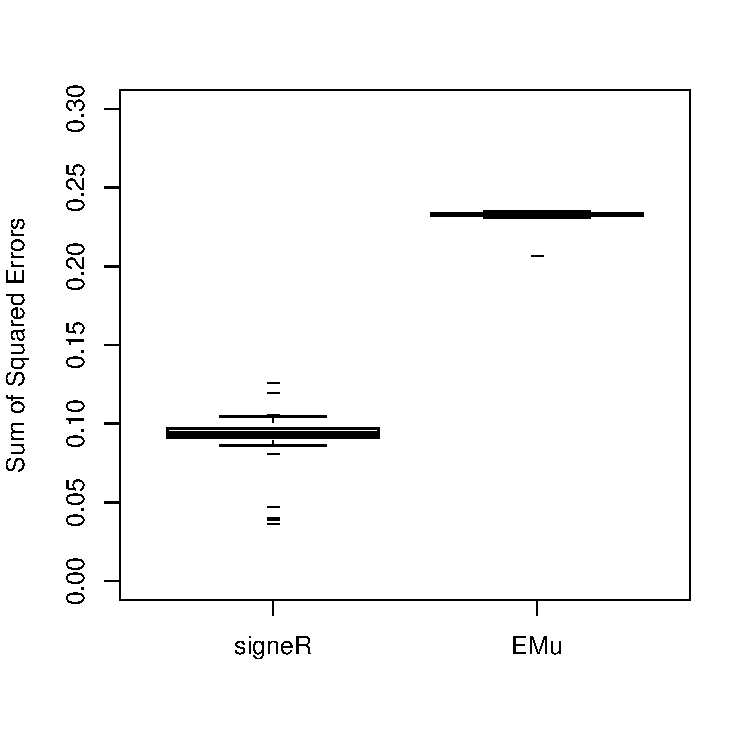
\includegraphics[width=6cm]{figs/Simulation_signeR_vs_EMu_boxplot_SSE}
   \\
 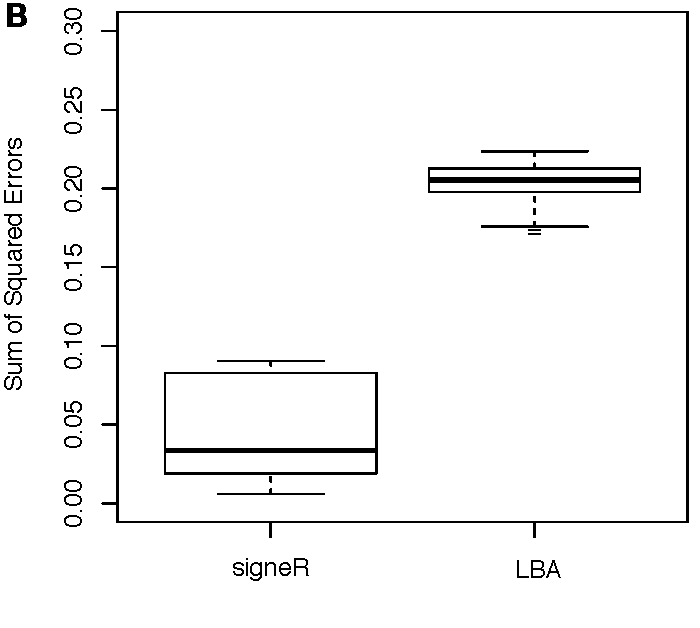
\includegraphics[width=6cm]{figs/Simulation_signeR_vs_Alex_boxplot_SSE_P}
   \end{tabular}
  \caption{\textrm{%
    Sum of squared errors for the estimated signatures. A:
    comparison between \texttt{signeR} and EMu by modelling a synthetic
    data set with opportunities. B: comparison between \texttt{signeR}
    and LBA by modelling a data set without opportunities.
   }
  }
  \label{fig:synth_SSE}
\end{figure}
\begin{figure}  
 \centering
  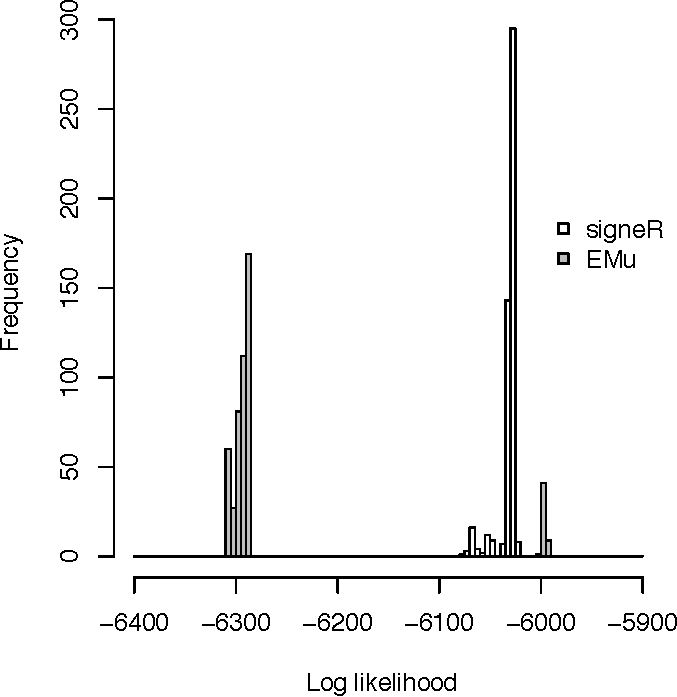
\includegraphics[width=6cm]{figs/Simulation_signeR_vs_EMu_histogram_LLh_same_axis_500sim} 
  \caption{\textrm{%
   Histogram of Log likelihood values at the estimates for $P$ and $E$
   obtained by the analysis of a 4 signatures synthetic data set via
   \texttt{signeR} and EMu. The analysis was made by including the
   mutation opportunity matrix $W$.
   }
  }
  \label{fig:synth_LLh}
\end{figure}

\section{Discussion}
The detection of mutational signatures from whole genome sequencing 
data has significantly advanced the understanding of mutagenesis and
the development of cancers. In this article we present a new method to
identify mutational signatures based upon an empirical Bayesian
treatment to the Poissonian NMF model. The empirical approach requires
minimal intervention form part of the user and is specially suited for
the applied practitioner.  A key aspect of our analysis
is that it addresses the model selection problem directly,
i.e. the estimation of the underlying number of signatures, without
using further approximations or ad hoc heuristics considered
previously. In addition, we introduce two concepts, namely the
Differential Exposure Score and posterior sample classification, which
may have potential impact in clinical practice.


The effectiveness of our method is shown by the analysis of real and
synthetic data sets. The results obtained with publicly available
data consisting of whole genome somatic mutations of 21 breast
cancers agree well with those in previous studies. Results obtained
with synthetic data show that our method presents several advantages
when compared to the two other techniques mostly used in the
literature and with the same NMF parameterisation as the one
considered here. When compared to \cite{FICMV}, our
method always estimates the correct number of signatures and even in
those cases where the former estimates the correct model dimension,
our estimates are more accurate. A comparison against the results
produced by \cite{A} with the correct dimension also shows that
our estimates are more accurate.

The estimation of the NMF rank is perhaps the most challenging
question regarding statistical inferences in the mutational signature
paradigm. Our approach to model choice relies on the use of the Bayes
Information criterion, which is a rough but simple approximation to
Bayesian factors, see \cite{KR}. These factors typically require the
computation of the marginal likelihood, defined as the normalising
constant of the posterior $\pi(Z, \theta_N, \psi_N|M, \eta, \Mord)$,
with $\Mord$ as the model indicator corresponding to the factorisation
rank $N$, and $\theta_N$ and $\psi_N$ respectively the associated
parameters and hyperparameters. By setting $\eta = \hat\eta$ and
conditioning on $\hat\eta$, Bayes theorem renders the marginal
likelihood as the ratio
\begin{equation}
  \label{eqn:Bfact}
   \ell(M|\hat \eta, \Mord) 
  = 
    \frac{p(M, Z, \theta_N, \psi_N|\hat\eta, \Mord)}
    {\pi(Z, \theta_N, \psi_N|M, \hat\eta, \Mord)},
\end{equation}
with $\eta$ fixed, contrary to what is assumed in definition of
$\mathcal L(\eta; m)$ by~(\ref{eqn:margLik}). The numerator is easily
computed by observing the conditional decomposition defined by the
hierarchical model. Indeed, this is simply given by
\[
%  p(M, Z, \theta_N, \psi_N|\hat\eta) 
%  = 
  p(Z, M|\theta_N, \psi_N, \Mord) p(\theta_N|\psi_N, \Mord)
  p(\psi_N|\hat\eta, \Mord).
\]
The evaluation of the denominator in (\ref{eqn:Bfact}) is however more
involved as it requires the joint posterior over the latent variables
and the parameters $\theta_N$ and $\psi_N$. This could be estimated at
any point of high probability by using the output from the MCMC EM
algorithm by using the approach suggested by \cite{Ch} or by other
means. Although promising, further work along these lines is
required.

\section*{Funding}
This work was partially supported by Funda\c{c}\~ao de Apoio a
Pesquisa do Estado de S\~ao Paulo (FAPESP), grant 15/19324-6. ED-N is
a research fellow from Conselho Nacional de Desenvolvimento Cientifico
e Tecnologico, Brazil (CNPq) and acknowledges the support received
from Associac\~ao Beneficente Alzira Denise Hertzog Silva (ABADHS) and 
FAPESP grant 14/26897-0.

%\bibliographystyle: natbib, achemnat, plainnat, abbrv, plain
\bibliographystyle{bioinformatics} 
\bibliography{bnmf}
\end{document}
%=-=-=-=-=-=-=-=-=-=-=-=-=-=-=-=-=-=-=-=-=-=-=-=-=-=-=-=-=-=-=-=-=-=
%%% Local Variables:
%%% mode: latex
%%% TeX-master: t
%%% End: